\documentclass[10pt]{article}

\usepackage[margin=0.75in]{geometry}
\usepackage{amsmath,amsthm,amssymb,bm}
\usepackage{xcolor}
\usepackage{cancel}
\usepackage{graphicx}
\usepackage{changepage}
\usepackage{circuitikz}
\usepackage{pgfplots}
\usepackage{minted}
\usepackage{physics}
\usepackage{hyperref}
\usepackage{siunitx}
\usepackage{fontspec}
\usepackage{relsize}
\usepackage{subfig}
\usepackage{todonotes}
\usepackage{multicol, multirow, booktabs}
\usepackage[breakable]{tcolorbox}
\usepackage[inline]{enumitem}

\theoremstyle{definition}
\newtheorem{problem}{Problem}
\newtheorem{soln}{Solution}

\pgfplotsset{compat=newest}
\usetikzlibrary{lindenmayersystems}
\usetikzlibrary{arrows}
\usetikzlibrary{calc}
\usetikzlibrary{positioning, fit}
\usetikzlibrary{3d, perspective}

\definecolor{incolor}{HTML}{303F9F}
\definecolor{outcolor}{HTML}{D84315}
\definecolor{cellborder}{HTML}{CFCFCF}
\definecolor{cellbackground}{HTML}{F7F7F7}
\newcommand{\ui}{\hat{i}}
\newcommand{\uj}{\hat{j}}
\newcommand{\uk}{\hat{k}}
\newcommand{\ux}{\hat{\mathbf{x}}}
\newcommand{\uy}{\hat{\mathbf{y}}}
\newcommand{\uz}{\hat{\mathbf{z}}}
\newcommand{\uv}[1]{\hat{\bv{{#1}}}}
\newcommand{\pr}[1]{{#1^\prime}}
\newcommand{\pd}[2][]{{\frac{\partial^{#1}}{\partial {{#2}^{#1}}}}}
\newcommand{\dif}[2][]{{\frac{d^{#1}}{d{{#2}^{#1}}}}}
\pgfdeclarelayer{background}  
\pgfsetlayers{background,main}
\AtBeginDocument{\RenewCommandCopy\qty\SI}

\makeatletter
\newcommand{\boxspacing}{\kern\kvtcb@left@rule\kern\kvtcb@boxsep}
\makeatother
\newcommand{\prompt}[4]{
    \ttfamily\llap{{\color{#2}[#3]:\hspace{3pt}#4}}\vspace{-\baselineskip}
}

\newcommand{\thevenin}[2]{
  \begin{center}
    \begin{circuitikz} \draw
      (0,0) -- (2,0) to[battery1, l_=$V_{Th}\eq#1$] (2,2) 
      to[resistor, l_=$R_{Th}\eq#2$] (0,2)
      ;
      \draw [o-] (-.07,2.079);
      \draw [o-] (-.07,0.079);
    \end{circuitikz}
  \end{center}
}

\newcommand{\norton}[2]{
  \begin{center}
    \begin{circuitikz} \draw
      (0,0) -- (3,0) to[american current source, l_=$I_{N}\eq#1$] (3,2) -- (0,2) (2,0)
      to[resistor, l=$R_{N}\eq#2$] (2,2)
      ;
      \draw [o-] (-.07,2.079);
      \draw [o-] (-.07,0.079);
    \end{circuitikz}
  \end{center}
}

\DeclareMathOperator{\Div}{div}
\DeclareMathOperator{\Curl}{curl}
\DeclareMathOperator{\sgn}{sgn}

\newcommand{\highlight}[1]{\colorbox{yellow}{$\displaystyle #1$}}

\newcommand{\ti}[1]{\widetilde{#1}}

\newfontface{\Kaufmann}{Kaufmann}
\DeclareTextFontCommand{\kf}{\Kaufmann}
\newcommand{\scriptr}{\fontsize{12pt}{12pt}\kf{r}}

\newfontface{\KaufmannB}{Kaufmann Bold}
\DeclareTextFontCommand{\kfb}{\KaufmannB}
\newcommand{\bscriptr}{\fontsize{12pt}{12pt}\kfb{r}}
\newcommand{\justif}[2]{&{#1}&\text{#2}}
\newcommand{\bv}[1]{\bm{\mathrm{#1}}}

\title{Physics 3200Y: Assignment V}
\author{Jeremy Favro (0805980) \\ Trent University, Peterborough, ON, Canada}
\date{\today}

\begin{document}
\maketitle


% CAPACITOR 2D - dielectric
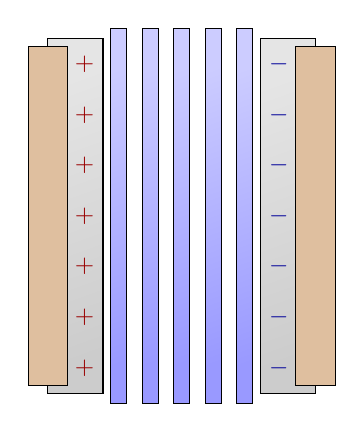
\begin{tikzpicture}
  \tikzstyle{dielectric}=[top color=blue!20,bottom color=blue!40,shading angle=20]
  \tikzstyle{foil}=[top color=gray!20,bottom color=gray!40,shading angle=20]
  \colorlet{pluscol}{red!60!black}
  \colorlet{minuscol}{blue!60!black}

  \def\H{4.5}
  \def\W{2.0}
  \def\w{0.7}
  \def\a{0.15*\W}
  \def\NE{6}
  \def\NQ{7}

  % DIELECTRIC
  \foreach \i [evaluate={\x=(\i-0.75)*\W/5}] in {1,...,5}{
      \draw[dielectric]
      (\x,-0.03*\H) rectangle (\x+0.1*\W,1.03*\H);
    }

  % PLATES
  \draw[foil]
  (0,0) rectangle++ (-\w,\H);
  \draw[fill=brown!50]
  (-0.45,0.1) rectangle ++(-\w+0.2,\H-0.2);

  \draw[foil]
  (\W,0) rectangle++ (\w,\H);
  \draw[fill=brown!50]
  (\W+0.45,0.1) rectangle ++(\w-0.2,\H-0.2);
  \foreach \i [evaluate={\y=(\i-0.5)*\H/\NQ;}] in {1,...,\NQ}{
      \node[pluscol,scale=0.9] at (-\w/3,\y) {$+$};
      \node[minuscol,scale=0.9] at (\W+\w/3,\y) {$-$};
    }
\end{tikzpicture}

\begin{circuitikz}
  \draw (0,0) to[sV=$V$] ++(0,-2) coordinate(V) to[capacitor, l=$C_s$] ++(0,-2) coordinate(J1) to[capacitor, l=$C_r$, voltage dir=RP, v=$V_r$]
  ++(0,-2) coordinate(J2) node[ground]{} ++(0,-1)
  (J1) -- ++(1.75,0) to[resistor, l=$R_{osc}$] ++(0,-2) -| (J2)
  (V) ++(0,1) to[open, voltage dir=RP, voltage/bump b =10, v=$V$] ++(0,-6)
  ;
\end{circuitikz}

\begin{tikzpicture}
  \begin{axis}[
      xmode=log,
      xlabel={Peak FFT Frequency (Hz)},
      ylabel={$C_s\,(\unit{\farad})$},
      legend style={at={(0.,0.02)},anchor=south west}
    ]
    \addplot table [x=freq (Hz), y=C_s (nF), col sep=comma] {0.17cm processed.csv};
    \addlegendentry{Dumy}
    \addplot table [x=freq (Hz), y=C_s (nF), col sep=comma] {0.3cm processed.csv};
    \addplot[mark=triangle*, brown] table [x=freq (Hz), y=C_s (nF), col sep=comma] {0.49cm processed.csv};
  \end{axis}
\end{tikzpicture}
\end{document}